\documentclass[UserManual.tex]{subfiles}
\begin{document}
\setcounter{section}{8}

\section{Underlying Theory of {\it Smooth Emulator}}\label{sec:theory}

The choice of model emulators, $E(\vec{\theta})$, depends on the prior understanding of the model being emulated, $M(\vec{\theta})$. If one knows that  a function is linear, then a linear fit is clearly the best choice. Whereas to reproduce lumpy features, where the lumps have a characteristic length scale, Gaussian process emulators are highly effective. The quality of an emulator can be assessed through the following criteria:
\begin{itemize}
  \item $E(\vec{\theta}_t)=M(\vec{\theta}_t)$ at the training points, $\vec{\theta}_t$. 
  \item The emulator should reasonably reproduce the model away from the training points. This should hold true for either interpolation or extrapolation.
  \item The emulator should reasonably represent its uncertainty
  \item A minimal number of training points should be needed
  \item The method should easily adjust to larger numbers of parameters, $\theta_i,~i=1\cdots N$
  \item The emulator should not be affected by unitary transformations of the parameter space
  \item The emulator should be able to account for noisy models
  \item Training and running the emulator should not be numerically intensive
\end{itemize}

Here the goal is to focus on a particular class of functions: functions that are {\it smooth}. Smoothness is a prior knowledge of the function. It is an expectation that the linear terms of the function are likely to provide more variance than the quadratic contributions, which are in turn likely to be more important than the cubic corrections, and so on. 

\subsection{Mathematical Form of {\it Smooth Emulator}}

To that end the following form for $E(\vec{\theta})$ is chosen,
\begin{align*}\eqnumber\label{eq:emudef}
E(\vec{\theta})&=\sum_{\vec{n}, {\rm s.t.}~K(\vec{n})\le K_{\rm max}} d_{\vec{n}}
f_{K(\vec{n})}(|\vec{\theta}|)
A_{\vec{n}}
\left(\frac{\theta_1}{\Lambda}\right)^{n_1}\left(\frac{\theta_2}{\Lambda}\right)^{n_2}\cdots 
\left(\frac{\theta_N}{\Lambda}\right)^{n_N}.
\end{align*}
Each term has a rank $K(\vec{n})=n_1+n_2+\cdots n_N$. If $f$ is constant, the rank of that term corresponds to the power of $|\vec{\theta}|/\Lambda$. All terms are included up to a given rank, $K_{\rm max}$. The coefficients $A$ are stochastically distributed. The coefficients $d_{\vec{n}}$ will ensure that the variance is independent of the direction of $\vec{\theta}$, with the constraint that $d_{K,0,0\cdots}=1$. The function $f_K(|\vec{\theta}|)$ provides the freedom to alter how the behavior depends on the distance from the origin, $|\vec{\theta}|$, and on the rank, $K$. Given that the variance of $A_{\vec{n}}$ can be changed, $f_{K=0}(|\vec{\theta}|=0)$ is also set to unity for all $K$ without loss of generality. For each combination $\vec{n}$, the prior probability for any the $A$ coefficients is given by 
\begin{align*}\eqnumber
p(A_{\vec{n}})&=\frac{1}{\sqrt{2\pi\sigma^2_{K(\vec{n})}}} e^{-A_{\vec{n}}^2/2\sigma_{K(\vec{n})}^2},\\
\langle A^2_{\vec{n}}\rangle&=\sigma^2_{K(\vec{n})}.
\end{align*}
The variance, $\sigma^2_K$, is allowed to vary as a function of $K$.

The parameter $\Lambda$ will be referred to as the {\it smoothness parameter}. Here, we assume that all parameters have a similar range, of order unity, e.g. $-1<\theta_i<1$. Thus, the relative importance of each term Eq. (\ref{eq:emudef}) falls with increasing rank, $K$, as $(1/\Lambda)^K$. For now, the smoothness parameter is fixed by prior knowledge, i.e. one chooses higher values of $\Lambda$ if one believes the function to be close to linear.

First, we consider the variance of the emulator at a given point, $\vec{\theta}$. Requiring that the variance is independent of the direction of $\vec{\theta}$ will fix $d_{\vec{n}}$.  For example, transforming $\theta_1$ and $\theta_2$ to parameters $(\theta_1\pm\theta_2)/\sqrt{2}$ should not affect the accuracy or uncertainty of the emulator.

At $|\vec{\theta}|=0$ the only term in Eq. (\ref{eq:emudef}) that contributes to the variance is the one $K=0$ term. Averaging over the $A$ coefficients, which can be either positive or negative with equal probability,
\begin{align*}\eqnumber
\langle E(\vec{\theta})\rangle=0,
\end{align*}
where the averaging refers to an average over the $A$ coefficients. At the origin, $|\vec{\theta}|=0$, the variance of $E$ is
\begin{align*}\eqnumber
\langle E(\theta_1=\theta_2=\cdots\theta_N=0)^2\rangle=d^2_{n_i=0}\sigma_{K=0}^2f_{K=0}^2(\vec{\theta}=0).
\end{align*}
Choosing $f_{K=0}(0)=1$ and $d_{n_i=0}=1$, the variance of $E$ is indeed $\sigma_0^2$. 
The variance at some point $\vec{\theta}\ne 0$ is 
\begin{align*}\eqnumber
\langle E^2(\vec{\theta})\rangle &=
\sum_{\vec{n}} 
f_K^2(|\vec{\theta}|)\sigma^2_{K(\vec{n})} d_{\vec{n}}^2
\left(\frac{\theta_1^{2n_1}}{\Lambda^2}\right)\left(\frac{\theta_2^{2n_2}}{\Lambda^2}\right)\cdots 
\left(\frac{\theta_N^{2n_N}}{\Lambda^2}\right).
\end{align*}
If $\langle E^2\rangle$ is to be independent of the direction of $\vec{\theta}$, the sum above must be a function of $|\vec{\theta}|^2$ only. This requires the net contribution from each rank, $K$ to be proportional to  $|\vec{\theta}|^{2K}$ multiplied by some function of $K$. Using the fact that
\begin{align*}\eqnumber
(\vec{\theta}_a\cdot \vec{\theta}_b)^K&=\sum_{\vec{n},s.t. \sum_i n_i=K}\frac{K!}{n_1!\cdots n_N!}(\theta_{a1}\theta_{b1})^{n_1}\cdots(\theta_{aN}\theta_{bN})^{n_N},
\end{align*}
one can see that if the sum is to depend only on the norm of $\vec{\theta}$,
\begin{align*}\eqnumber
d_{\vec{n}}^2&=\frac{K(\vec{n})!}{n_1!n_2!\cdots n_N!}.
\end{align*}
The factor of $K!$ in the numerator was chosen to satisfy the condition that $d_{K,0,0,0}=1$.

One can now calculate the correlation between the emulator at two different points, averaged over all possible values of $A$,
\begin{align*}\eqnumber
\langle E(\vec{\theta}_a)E(\vec{\theta}_b)\rangle &=
\sum_{K=0}^{K_{\rm max}}\sigma_K^2f_K^2(|\vec{\theta}|)
\left(\frac{\vec{\theta}_a\cdot\vec{\theta}_b}{\Lambda^2}\right)^{K}.
\end{align*}
Requiring $f(|\theta|=0)=1$ gives
\begin{align*}\eqnumber
\langle E^2(\vec{\theta}=0))\rangle &=\sigma_0^2,
\end{align*}
and for $\vec{\theta}_a=\vec{\theta}_b$,
\begin{eqnarray}
\langle E^2(\vec{\theta}=0))\rangle &=\sum_{K=0}^{K_{\rm max}}
\sigma_K^2f_K^2(|\vec{\theta}|)\left(\frac{|\vec{\theta}|^2}{\Lambda^2}\right)^K.
\end{eqnarray}

To this point, the form is completely general once one requires that the variance above is independent of the direction of $\vec{\theta}$. I.e. the function $f_K(\vec{\theta})$ could be any function satisfying the constraint, $f_K(0)=1$, and $\sigma_K^2$ could have any function of $K$. Below, we illustrate how different choices for $f$ or for $\sigma_K$ affect the emulator by comparing several variations. First, we define the default form.

\subsection{Alternate Forms}
As stated above, once the form is to provide variances that are independent of the direction of $\vec{\theta}$, the general form going forward is
\begin{align*}\eqnumber
E(\vec{\theta})&=\sum_{\vec{n},{\rm s.t.}~K(\vec{n})<K_{\rm max}}
f_{K}(|\vec{\theta}|)
\left(\frac{K(\vec{n})!}{n_1!\cdots n_N!}\right)^{1/2}
A_{\vec{n}}
\left(\frac{\theta_1}{\Lambda}\right)^{n_1}
\left(\frac{\theta_2}{\Lambda}\right)^{n_2}
\cdots 
\left(\frac{\theta_N}{\Lambda}\right)^{n_N},\\
P(\vec{A}_n)&=\frac{1}{(2\pi\sigma_K^2)^{1/2}}e^{-|A_{\vec{n}}|^2/2\sigma_K^2}.
\end{align*}
Variations from the general form involve adjusting either the $K$-dependence of the $|\vec{\theta}|$-dependence of $f_K(|\vec{\theta}|)$, or adjusting the $K$-dependence of $\sigma_K$.

\noindent{\bf Default Form}\\
Here, we assume $f_K(|\vec{\theta}|)$ is independent of $|\vec{\theta}|$, and that $\sigma_K$ is independent of $K$. Further, the $K-$dependence of $f^2$ is assumed to be $1/K!$. With this choice
\begin{align*}\eqnumber
E(\vec{\theta})&=\sum_{\vec{n},K(\vec{n})\le K_{\rm max}}\frac{1}{\Lambda^K}\frac{A_{\vec{n}}}{\sqrt{n_1!n_2!\cdots n_N!}}
\theta_1^{n_1}\cdots\theta_N^{n_N},\\
P(A_{\vec{n}})&\sim e^{-A^2_{\vec{n}}/2\sigma^2}.
\end{align*}
With this form the variance increases with $|\vec{\theta}|$,
\begin{eqnarray}
\langle E^2(\vec{\theta})\rangle&=\sigma^2e^{|\vec{\theta}|^2/\sigma^2}.
\end{eqnarray}
If the function is trained in a region where the function is linear, the emulator's extrapolation outside the region will continue to be follow the linear behavior, albeit with variation from the higher order coefficients.

The choice of $f^2_K=1/K!$ ensures that the sum defining $E(\vec{\theta})$ converges as a function of $K$ as long as $K_{\rm max}$ is rather large compared to $|\vec{\theta}|/\Lambda$. 

\noindent{\bf Variant A: Letting $\sigma_K$ have a $K$ dependence}\\
One reasonable alteration to the default choice might be to allow the $K=0$ term to take any value, i.e. $\sigma_{K=0}=\infty$, while setting all the other $\sigma_K$ terms equal to one another. This would make sense if our prior expectation of smoothness meant that we expect the $K=2$ terms to be less important than the $K=1$ terms, by some factor $|\vec{\theta}|/\Lambda$, but that the variation of the $K=1$ term is unrelated to the size of the $K=0$ term. This would make the emulator independent of redefinition of the emulated function by adding a constant. This may well be a reasonable choice for many circumstances.

\noindent{\bf Variant B: Suppressing  correlations for large $\Delta\vec{\theta}$}\\
This form for $f$ causes correlations to fall for points far removed from one another. 
\begin{align*}\label{eq:fform}
f_K(|\vec{\theta}|)&=\frac{1}{\sqrt{K!}}\left\{
\sum_{K=0}^{K_{\rm max}}\frac{1}{\sqrt{K!}}\left(\frac{|\vec{\theta}|^2}{2\Lambda^2}\right)^K\right\}^{-1/2}.
\end{align*}
In the limit that $K_{\rm max}\rightarrow\infty$ the form is a simple exponential,
\begin{align*}\eqnumber
\left.f_K(|\vec{\theta}|)\right|_{K_{\rm max}\rightarrow\infty}&=
\frac{1}{\sqrt{K!}}e^{-|\vec{\theta}|^2/2\Lambda^2}.
\end{align*}
With this form the same-point correlations remain constant over all $\vec{\theta}$,
\begin{align*}\eqnumber
\langle E(\vec{\theta})E(\vec{\theta})\rangle&=\sigma^2,
\end{align*}
while the correlation between separate positions fall with increasing separation. This is especially transparent for the $K_{\rm max}\rightarrow\infty$ limit,
\begin{align*}
\langle E(\vec{\theta}_a)E(\vec{\theta}_b)\rangle_{K_{\rm max}\rightarrow\infty}
&=\sigma^2 e^{-|\vec{\theta}_a-\vec{\theta}_b|^2/2\Lambda^2}.
\end{align*}
In this limit one can also see that
\begin{align*}\eqnumber
\langle[E(\vec{\theta})-E(\vec{\theta}')]^2\rangle_{K_{\rm max}\rightarrow\infty}&=
2\sigma^2\left(1-e^{|\vec{\theta}-\vec{\theta}'|^2/2\Lambda^2}\right).
\end{align*}
If one trains such an emulator in one region, then extrapolates to a region separated by $|\vec{\theta}-\vec{\theta}'|>>\Lambda$, the average predictions will return to zero. Thus, if the behavior would appear linear in some region the emulator's distribution of predictions far away (extrapolations) would center at zero. This behavior is similar to a Gaussian-process emulator.

\noindent{\bf Variant C: Eliminating the $1/K!$ weight}\\
Clearly, eliminating the $1/K!$ weights in $f_K$ would more emphasize the contributions from larger $K$. But, for and $|\vec{\theta}|>\Lambda$ the contribution to the variance would increase as $K$ increases and the sum would not converge if $K_{\rm max}$ were allowed to approach infinity. An example of a function that expands without factorial suppression is $1/(1-x)=1+x+x^2+x^3\cdots$, which diverges as $x\rightarrow 1$. If such behavior is not expected, then this choice would be unreasonable.

\subsection{Tuning the Emulator}

Here, we illustrate how an emulator of the form above can be constrained given training points. We consider $M$ full model runs at positions $\vec{\theta}_{m=1,M}$, with values $F_{m=1,M}$. The functional form has a large number of coefficients, $A_{\vec{n}}$, which is much larger than the number of training points, $M$. However, the dependence of $A$ is purely linear. One can enumerate the coefficients as $A_c$ with $c=1\cdots C$, where $C>M$. One can randomly set the coefficients $A_M$ through $A_C$, then solve for the first $M$ coefficients by solving a linear equation. One can then apply a weight based on the values of $A$ consistent with the prior likelihood of $A$ and the constraints. One can then generate a representative set of $A$, perhaps a dozen samples. Each sample function will go through all the training points, but will vary further from the training points. Averaging over the $N_{\rm sample}$ sets of coefficients can be used to make a prediction for the emulator at some point $\vec{\theta}$, and the variance of those $N_{\rm sample}$ points would represent the uncertainty of the emulator.

Here, we present two different methods for generating samples of points that are consistent with the training constraints and with the prior range of parameters. We do this for the default method, but this can be easily extended to the other model variants listed in the previous section. In addition to varying the coefficients, we will additionally vary the width parameters, $\sigma$.

First, we need to describe how the weights are generated. The probability of a set of coefficients is initially 
\begin{align*}\eqnumber
P(A_c)&=\frac{1}{\sqrt{2\pi \sigma^2}}e^{-A_c^2/2\sigma^2}.
\end{align*}
If we also vary $\sigma$, we can state that 
\begin{align*}\eqnumber
Q(\sigma)&=\frac{1}{\pi}\frac{\Gamma/2}{\sigma^2+(\Gamma/2)^2}.
\end{align*}
Here, the half width of the distribution should be set to some large value to encompass the degree to which the emulated function might vary. The Lorentzian form accommodates a large uncertainty. The result should not depend strongly on $\Gamma$. The joint probability is $Q(\sigma)\prod_c P(A_c)$. 

The constrained probability is
\begin{align*}\eqnumber
dP&=d\sigma Q(\sigma)\prod_c[dA_c~P(A_c)]\prod_{m=1}^M \delta(E(A,\sigma,\vec{\theta}_m)-F(\vec{\theta}_m))\\
&=d\sigma Q(\sigma) \prod_{c=1}{^M}P(A_c)\frac{1}{|J|} \prod_{c=M}^C [dA_c~P(A_c)].
\end{align*}
Here, $|J|$ is the Jacobian, i.e. it is the determinant of the $M\times M$ matrix
\begin{align*}\eqnumber
J_{mc}&=\frac{\partial E(\vec{\theta}_m)}{\partial A_c},
\end{align*}
For the default form in the previous section,
\begin{eqnarray}
J_{mc}&=\frac{1}{\sqrt{n_{c1}!\cdots n_{cN}!}}(\theta_{m1})^{n_{c1}}\cdots(\theta_{mN})^{n_{cN}}.
\end{eqnarray}
Because the Jacobian depends only on the position of the training points, it can be treated as a constant. 

One can now sample $A$ and $\sigma$ according to the weights above. Here, we list two methods.

\begin{itemize}\itemsep=0pt
\item [a)] {\bf Keep and Reject Method}\\
One can generate the coefficients $A_{c=M}\cdots A_{C}$ according to the Gaussian distribution with width $\sigma$, after generating $\sigma$ according to the Lorentzian. The residual weight is then
\begin{align*}\eqnumber
w&=\prod_{c=1}{^M}P(A_c).
\end{align*}
For each attempt, one could keep or reject the attempt with probability $w$. This generates perfectly independent samples, but with the caveat that in a high dimensional space the rejection level might be quite high.
\item [b)] {\bf Metropolis Exploration of $A$ and $\sigma$}\\
Beginning with any configuration $A$ and width $\sigma$, one can take a random step $\delta A$ and $\delta\sigma$. In the absence of any weight this would consider all $A$ or $\sigma$ with values from $-\infty$ to $\infty$. The residual weight would then be
\begin{align*}\eqnumber
w&=Q(\sigma)\prod_{c=1}^C P(A_c).
\end{align*}
One then keeps the step if the new weight exceeds the previous one, or if the ratio of the new weight to the old weight is greater than a random number between zero and unity. After some number of steps, $N_{\rm steps}$, one saves the configuration as a representative sample for the emulator. The disadvantage of this approach is that many steps may be needed to ensure that the samples are independent, and thus faithfully represent the variation in the emulator.
\end{itemize}

\section{Theoretical Basis of {\it Simplex Sampler}}\label{sec:simplextheory}

Here, we imagine a spherically symmetric prior, e.g. one that is purely Gaussian, and where the parameters are scaled so that the prior distribution is invariant to rotations. If one believe the function were close to linear, a strategy would be to find $M=N+1$ points in parameter space placed far apart from another. One choice is the $N-$dimensional simplex. Examples are an equilateral triangle in two-dimensions or a tetrahedron in three dimensions. For a simplex, one places the $M=N+1$ training points at a uniform distance from the origin, $r$, with equal separation between each point. One can generate an $N-$dimensional simplex from an $N-1$ dimensional arrangement. In the $N-1$ dimensional arrangement, the points are arranged equidistant from one another using the coordinates $x_1\cdots x_{N}$. The points would all be placed at a radius $r_{N}$ from the origin in this system, and the separation would be $d$. In the $N-$dimensional system all these $N-1$ points had coordinate $x_N=-a$. The $(N+1)^{\rm th}$ point is then placed at position $x_1\cdots x_{N}=0$ and $x_{N+1}=Na$. This keeps the center of mass at zero. One then chooses $a$ such that the new point is equally separated from all the other points by the same distance $d$, 
\begin{align*}\eqnumber
d^2&=r_{N-1}^2+N^2a^2,\\
a&=\sqrt{\frac{d^2}{N^2}-r_{N-1}^2}.
\end{align*}
Now, each of the $N$ points is located a distance $Na$ away from the center of the $N-$dimensional origin. This procedure can applied iteratively to generate the vertices of the simplex.

One might also wish to use enough training points to uniquely determine the emulator in the case that the function is quadratic. There are $N(N+1)/2$ additional points, which is exactly the number of segments connecting the $N+1$ equally-spaced vertices of the  $N-$dimensional simplex. If placed at the midpoints of the segments, these points would be closer to the  origin than the vertices. One of the simplex options is to place these points at the midpoints, then double their radii while maintaining their direction. This would result in arrays of points at two different radii, with $N+1$ points positioned at the lower radius and $N(N+1)/2$ points being placed at the larger radius.

Choosing the training points depends on prior expectation of the emulated function. The simplex choice for the first $M=N+1$ points seems logical. Even if another method, such as a Gaussian process emulator is to implemented, such methods are often based on first understanding the linear behavior. The simplex strategy would seem a good way to pick the first $N+1$ training points.

One issue with the simplex is that the first set of $N+1$ training points would all be placed at the same radius. If the prior parameter distribution is uniform within an $N-$dimensional hyper cube, the training  points could be rather far from the corners in that space. Issues with such priors are discussed in the next section.

\subsection{The Pernicious Nature of Step-Function Priors in High Dimension}

For purely Gaussian priors, one can scale the prior parameter space to be spherically symmetric. Unfortunately, that is not true for step function priors (uniform within some range). In that case the best one can do (if the priors for each parameter are independent) is to scale the parameter space such that each parameter has the constraint, $-1<\theta_i<1$. If the number of parameters is $N$, the hyper-cube has $2N$ faces and $2^N$ corners, a face being defined as one parameter being $\pm 1$ while the others are zero, while a corner has each parameter either $\pm 1$. For 10 parameters, there are 1024 corners, and for 15 parameters there are 32678 corners. Thus, it might be untenable to place a training point in each corner. 

One can also see the problem with placing the training points in a spherically symmetric fashion as is done with the {\it Simplex Sampler}. The hyper-volume of the parameter-space hyper-cube is $2^N$, whereas the volume of an $N-$dimensional hyper-sphere of radius $R=1$ is 
\begin{align*}\eqnumber
V_{\rm sphere}=\Omega_N\int_0^R dr~r^{N-1}=\Omega_N\frac{R^N}{N}.
\end{align*}
The solid angle, $\Omega_N$ in $N$ dimensions is
\begin{align*}\eqnumber
\Omega_N&=\frac{2\pi^{N/2}}{\Gamma(N/2)},
\end{align*}
and after putting this together, the fraction of the hyper-cube's volume that is within the hyper-sphere is
\begin{align*}\eqnumber
\frac{V_{\rm sphere}}{V_{\rm cube}}&=\left\{\begin{array}{rl}
\frac{(\pi/2)^{N/2}}{N!!},&N=2,4,6,8\cdots\\
\frac{(\pi/2)^{(N-1)/2}}{N!!},&N=3,5,7,\cdots\end{array}\right.
\end{align*}
In two dimensions, the ratio is $\pi/4$, and in three dimensions it is $\pi/6$. In 10 dimensions it is $2.5\times 10^{-3}$. For high dimensions only a small fraction of the parameter space can ever lie inside inside a sphere used to place points. And, if the model is expensive, it may not be tenable to run the full model inside every corner. 

One can also appreciate the scope of the problem by considering the radius of the corners vs. the radius of  the sphere. The maximum value of $|\vec{\theta}|$ is $\sqrt{N}$. So, for 9 parameters, if the  training points were all located at positions $|\vec{\theta}|<1$, one would have to extrapolate all the way to $|\vec{\theta}|=3$. Thus, unless the model is exceptionally smooth, one needs to devise a strategy to isolate the portion of likely parameter space using some original set of full-model runs, then augment those runs in the likely region. 

A third handle for viewing the issue in $N$ dimensions is to compare the r.m.s. radii of the hyper-sphere to that of the hyper-cube. For the cube where each side has length $2a$,
\begin{align*}\eqnumber
\left(R_{\rm r.m.s.}^{\rm(cube)}\right)^2&=a^2\frac{N}{3}.
\end{align*}
whereas for a sphere of radius $a$,
\begin{align*}\eqnumber
\left(R_{\rm r.m.s.}^{\rm(sphere)}\right)^2&=a^2\frac{N+2}{N}.
\end{align*}
The ratio of the radii is then
\begin{align*}\eqnumber
\frac{R_{\rm r.m.s.}^{\rm(sphere)}}{R_{\rm r.m.s.}^{\rm(cube)}}&=\sqrt{\frac{3}{N+2}}.
\end{align*}
Thus, in 10 dimensions, if the training points are placed at a distance $a$ from the origin, the r.m.s. radii of the interior space would be half that of the entire space. Further, the r.m.s. radii of the points in the cube, $a\sqrt{N/3}$, would be about 83\% higher than the radius of the training points. 

Of course, these problems would be largely avoided if the number of parameters was a half dozen or fewer, or if one was confident that the function was extremely smooth. In the first two sections of this paper, the smoothness parameter, $\Lambda$, was set to a constant. There might be prior knowledge that certain parameters affect the observables only weakly. In that case, the response to these parameters can be considered as linear. This could be done by scaling those parameters so that they vary over a smaller range. If a parameter varies only between $-0.1$ and $0.1$, that effectively applies a smoothness parameter in those directions that is ten times higher. Unfortunately, the choice of which parameters to rescale in this fashion would likely vary depending on which observable is being emulated. Because all the observables might be calculated in a full model run, one needs to identify parameters that would likely have weak response on all observables. 

\section{Tests of the {\it Smooth Emulator} using {\it Simplex Sampler} for Training}

First, we show some results of one-parameter emulators. For a linear fit, two parameters (slope and intercept) would suffice. But because higher-rank contributions exist, there is a spread of functions is that narrows with increasing smoothness parameter as shown in Fig. \ref{fig:onedim}. Figure \ref{fig:onedim} also shows how increasing the number of training points, from two to three, also narrows the range of possible values. 
\begin{figure}
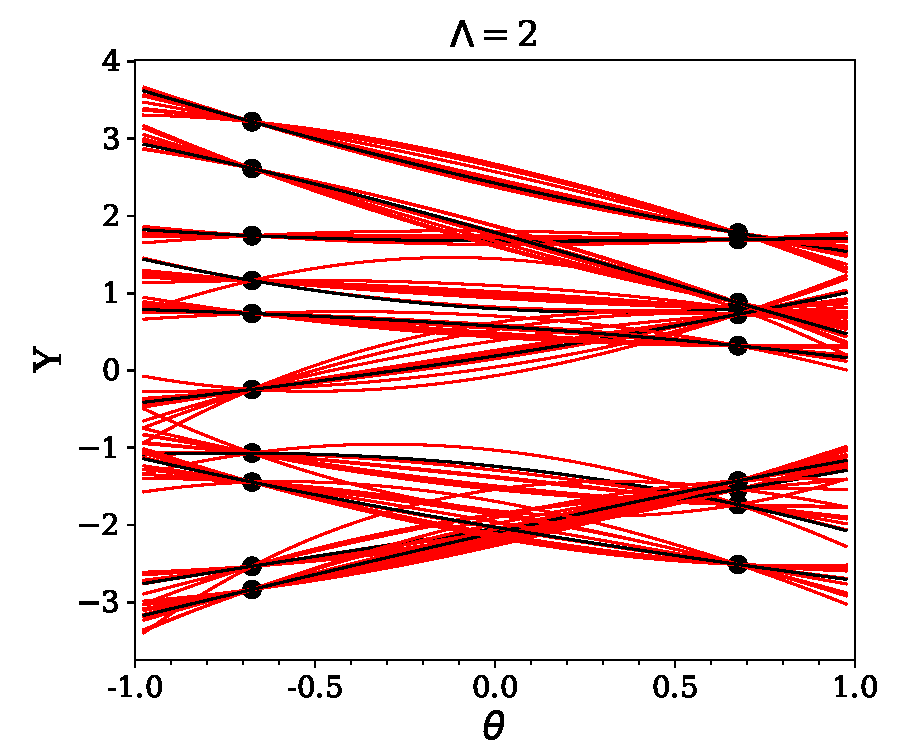
\includegraphics[width=0.32\textwidth]{onepar2points/onepartest_Lambda2}\hspace*{0.02\textwidth}
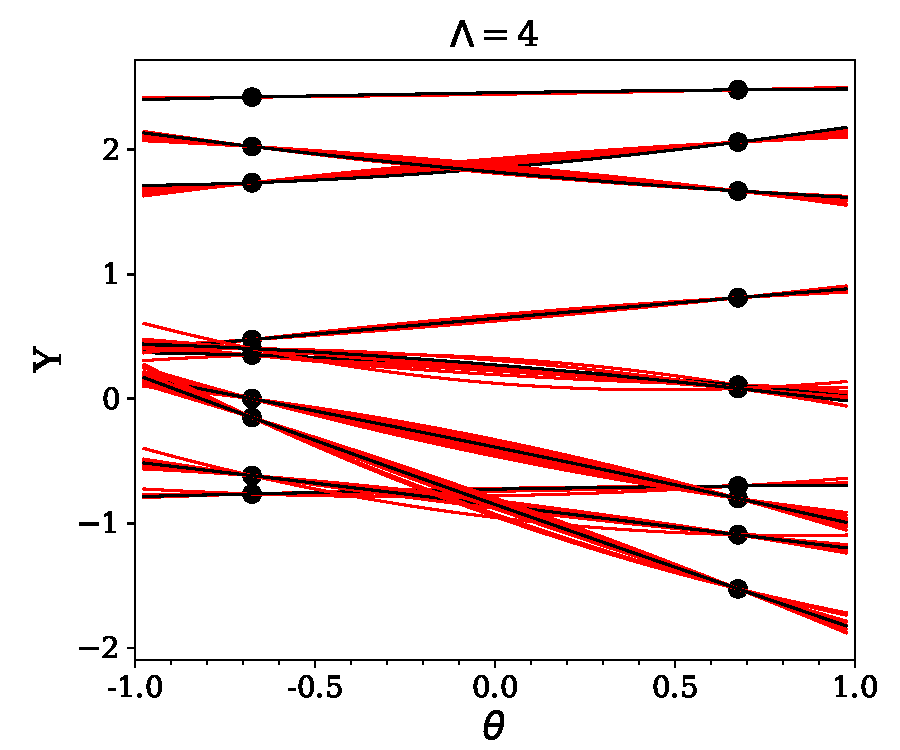
\includegraphics[width=0.32\textwidth]{onepar2points/onepartest_Lambda4}\hspace*{0.02\textwidth}
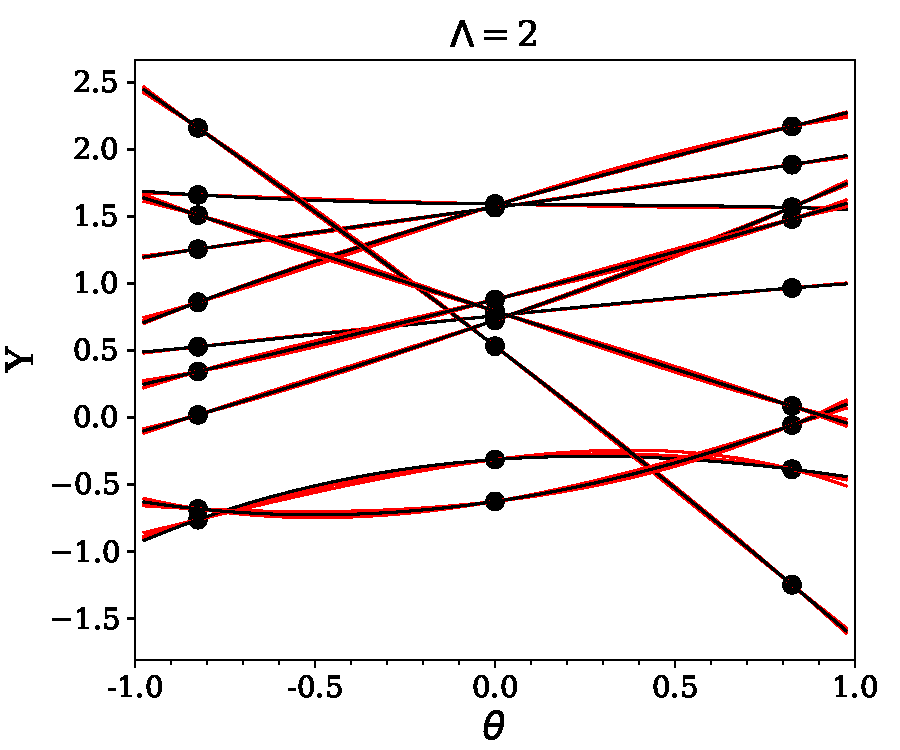
\includegraphics[width=0.32\textwidth]{onepar3points/onepartest_Lambda2}
\caption{\label{fig:onedim}
Real functions (black lines) are emulated with the {\it Smooth Emulator} (default settings). Ten different functions are emulated. Each emulation is sampled ten times (red lines), with the spread of the lines representing the uncertainty.}
\end{figure}

Next, we repeat the same test with six parameters. The prior distribution of parameters was uniform in the region $-1<\theta_i<1$. In this case, the {\it Simplex Sampler} was used to choose the training points. The ``real'' model, $F$, was constructed from sample smooth functions, with the coefficients generated randomly and a smoothness parameter set to three or six. The $A_{\vec{n}=0}$ coefficient for the real model was set to zero to better accommodate viewing results. The emulator was not given that information. Twenty instances of real models were emulated. For each real model five random point in parameter space were chosen. The emulator value and its uncertainty are plotted alongside the real-model values in Fig. \ref{fig:sixpars}. The 100 comparisons show that the emulator accurately predicts the uncertainty. This is not surprising, because the emulator used the same smoothness parameter as was used to construct the real models. The width parameters, $\sigma$, were explored stochastically, and remarkably they seem to fluctuate around the same value used to construct the real model, albeit with fluctuations of the order of 30\%. 

Figure \ref{fig:sixpars} first shows the 100 comparisons for the case with the smoothness parameter, $\Lambda=3$. The simplest simplex form was applied, which has seven parameters, the same number one would use for a linear fit. Uncertainties were provided by finding 16 independent samplings of $A$ coefficients and of $\sigma$, then using the variance of the 16 samples to define the uncertainty. Variant {\it a} of the default emulator was used, i.e. the coefficient $A_0$ was not given a constraining prior distribution, whereas all other coefficients were weight by a Gaussian of width $\sigma$. In the other two panels of Fig. \ref{fig:sixpars}, the procedure was repeated but once with a higher smoothness parameter, and once with a the 28 training points, placed according to the procedure mentioned in Sec. \ref{sec:simplex}, where an additional set of points in parameter space was generated by choosing points that bisect all the lines connecting points in the original simplex, then doubling their radius. As expected, smoother functions are more easily emulated with a given number of training points, and using more training points also improves the accuracy. 
\begin{figure}
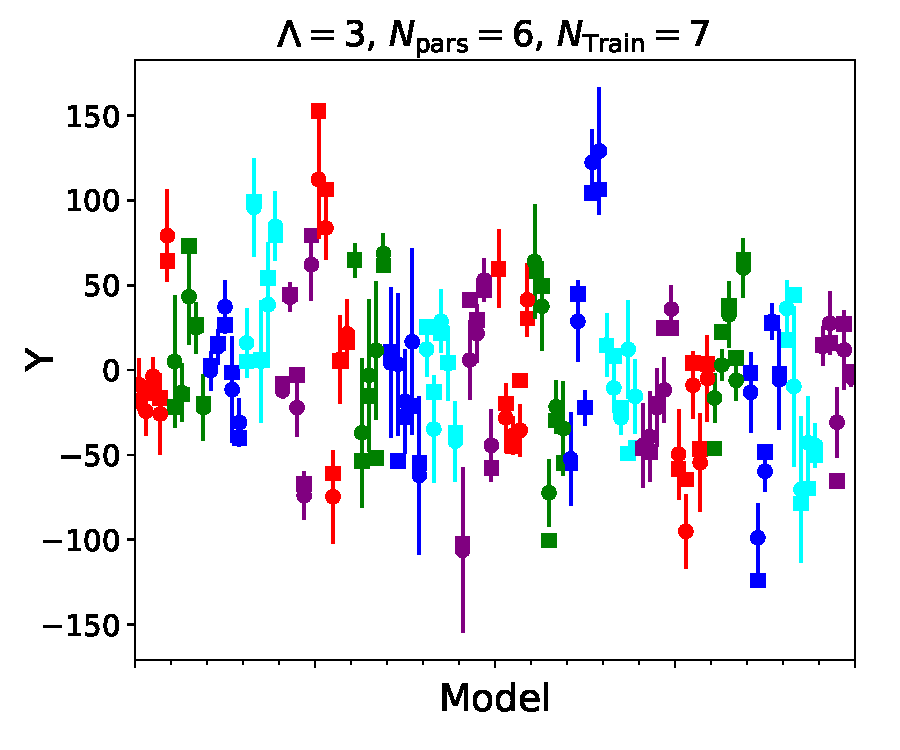
\includegraphics[width=0.32\textwidth]{sixpars/NPars6_Lambda3_NTrain7}\hspace*{0.02\textwidth}
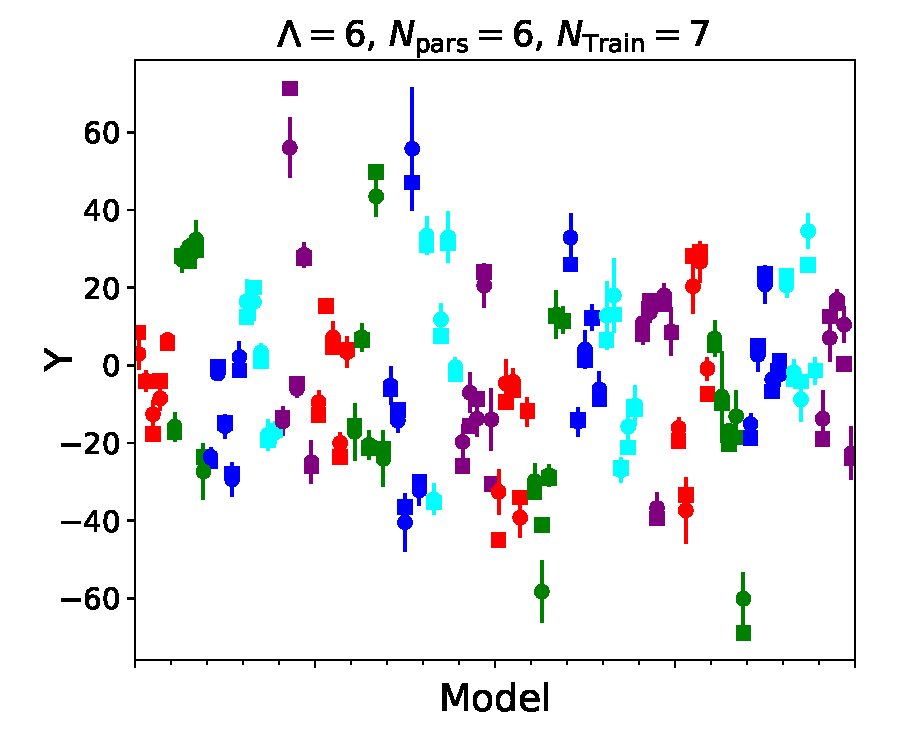
\includegraphics[width=0.32\textwidth]{sixpars/NPars6_Lambda6_NTrain7}\hspace*{0.02\textwidth}
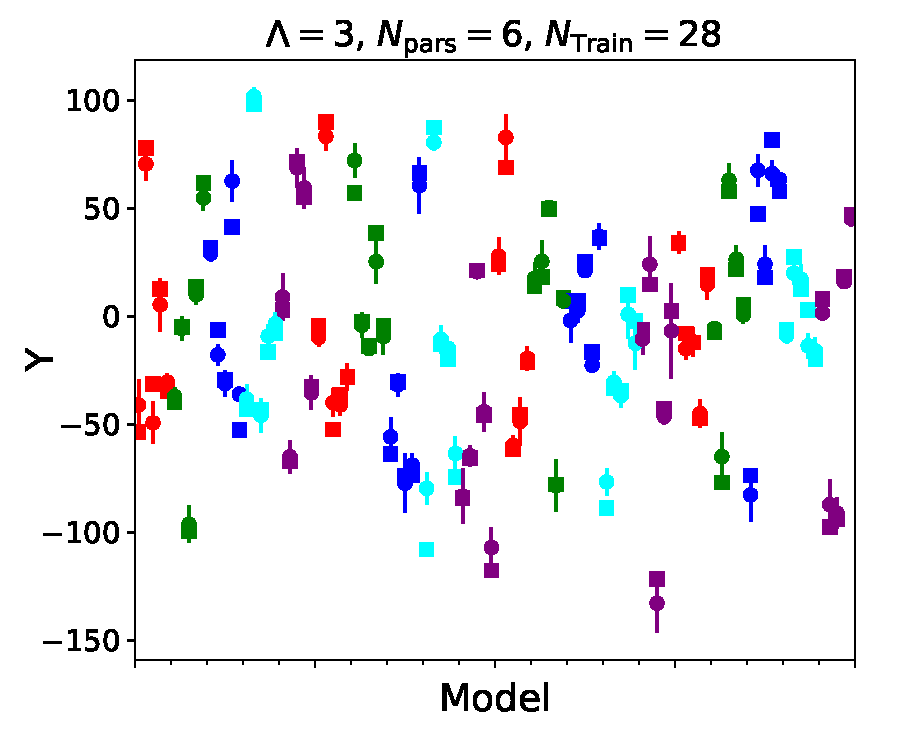
\includegraphics[width=0.32\textwidth]{sixpars/NPars6_Lambda3_NTrain28}
\caption{\label{fig:sixpars}
Using 20 instances of real models using six parameters, choosing 5 random points in parameter space for each model, the emulator (circles) and its uncertainty were compared to the real values (squares). Neighboring points of the same color emulated the same real model. The accuracy improves if a smoother function is considered (middle panel), or if more training points are used (right panel). Estimates of the uncertainty seem reasonable given that the uncertainties illustrated in the figure represent one standard deviation. It should be emphasized that this consistency depends critically on the fact that the emulator chose the same smoothness parameter as was used to generate the real models.
}
\end{figure}

\end{document}
